% OWD 2024: IMLO assignment report
%
\documentclass[journal]{IEEEtran}
\usepackage[en-GB]{datetime2}
\usepackage{xcolor, amsmath, amssymb, tikz}
\usepackage{pgfplots}
\usepackage[
    colorlinks,
    linkcolor={red!50!black},
    citecolor={blue!50!black},
    urlcolor={blue!80!black}
]{hyperref}

\usetikzlibrary{positioning, fit}
\pgfplotsset{compat=1.18}

\newcommand\dotsep{\enspace\textperiodcentered\enspace}
\DeclareMathOperator\relu{\mathsf{ReLU}}
\DeclareMathOperator\batchnorm{\mathsf{BNorm}}
\DeclareMathOperator\linear{\mathsf{Lin}}
\DeclareMathOperator\loss{\mathsf{SCELoss}}
\DeclareMathOperator\convol{\mathsf{Conv2d}}
\DeclareMathOperator\weight{\mathsf{Weight}}
\DeclareMathOperator\maxpool{\mathsf{MaxPool2d}}
\DeclareMathOperator\bias{\mathsf{Bias}}

\newcommand\networkperformance{43}
\newcommand\trainingtime{\textbf{TODO}}
\newcommand\trainingepochcount{\textbf{TODO}}

\newcommand\candidate{Examination Candidate \#Y3898772}
\title{Classification of the 102-Category \emph{Flowers} Dataset with
    Convolutional Deep Neural Networks}
\author{\candidate%
    \thanks{Manuscript prepared with \LaTeX\ and \texttt{IEEEtran} on \today.}%
    \thanks{All submitted work, unless stated otherwise, is the sole creation
    of \candidate.}}

\IEEEspecialpapernotice{Submitted in partial fulfilment of the requirements of
    the \href{https://www.york.ac.uk/students/studying/manage/programmes/%
    module-catalogue/module/COM00026I/2023-24}{\emph{Intelligent Systems:
    Machine Learning and Optimisation}} module assignment at the University of
    York in the 2023/24 academic year.\vspace{-2ex}}

\begin{document}
\maketitle
\begin{figure*}[t]
    % This figure must be defined on the page preceding its intended ship-out.
    \pgfdeclarelayer{nnlayerbound}
\pgfdeclarelayer{nnlayercontent}
\pgfdeclarelayer{nnlayerarrow}
\pgfsetlayers{nnlayerbound, nnlayercontent, nnlayerarrow}
%
\begin{tikzpicture}
    \def\hpad{.5cm}
    \def\vpad{1.3cm}

    \begin{pgfonlayer}{nnlayercontent}
    \begin{scope}[every node/.append style={draw, minimum height=2em,
            fill=white}] % Fill with white so that the layering is visible
        \node (in) {\color{red}{Input ($4 \times 3 \times 224 \times 224$)}};

        \node [right = \hpad of in]    (conv1) {$\convol$ ($3$ / $32$)};
        \node [right = \hpad of conv1]   (bn1) {$\batchnorm$};
        \node [right = \hpad of bn1]   (relu1) {$\relu$};
        \node [right = \hpad of relu1] (pool1) {$\maxpool$};

        \node [right = \hpad of pool1] (conv2) {$\convol$ ($32$ / $64$)};
        \node [right = \hpad of conv2]   (bn2) {$\batchnorm$};
        \node [below = \vpad of bn2.east, anchor=east]
            (relu2) {$\relu$};
        \node [left  = \hpad of relu2] (pool2) {$\maxpool$};

        \node [left =  \hpad of pool2] (conv3) {$\convol$ ($64$ / $128$)};
        \node [left  = \hpad of conv3]   (bn3) {$\batchnorm$};
        \node [left  = \hpad of bn3]   (relu3) {$\relu$};
        \node [left  = \hpad of relu3] (pool3) {$\maxpool$};

        \node [left  = \hpad of pool3]   (lin1) {$\linear$ ($86528$ / $2048$)};
        \node [left  = \hpad of lin1]   (relu4) {$\relu$};

        \node [below = \vpad of relu4.west, anchor=west]
            (lin2) {$\linear$ ($2048$ / $1024$)};
        \node [right = \hpad of lin2] (relu5) {$\relu$};

        \node [right = \hpad of relu5] (lin3) {$\linear$ ($1024$ / $512$)};
        \node [right = \hpad of lin3] (relu6) {$\relu$};

        \node [right = \hpad of relu6]  (lin4) {$\linear$ ($512$ / $102$)};
        \node [right = \hpad of lin4]  (relu7) {$\relu$};

        \node[right = \hpad of relu7] (out)
            {\color{red}{Output ($4 \times 102$)}};
    \end{scope}
    \end{pgfonlayer}

    % Draw CONV-BN-RELU-POOL layer bounding boxes and intra-layer arrows
    \foreach \layeridx in {1, 2, 3} {
        \begin{pgfonlayer}{nnlayerbound}
            \node[draw, lightgray, dashed, fit=
                (conv\layeridx) (bn\layeridx)
                (relu\layeridx) (pool\layeridx)]
                {};
        \end{pgfonlayer}

        \begin{pgfonlayer}{nnlayerarrow}
            \draw[-latex] (conv\layeridx) -- (bn\layeridx);
            \draw[-latex] (bn\layeridx)   -- (relu\layeridx);
            \draw[-latex] (relu\layeridx) -- (pool\layeridx);
        \end{pgfonlayer}
    }

    % Inter-layer arrows for CONV-BN-RELU-POOL layers
    \begin{pgfonlayer}{nnlayerarrow}
        \draw[-latex, red] (pool1) -- (conv2);
        \draw[-latex, red] (pool2) -- (conv3);
        \draw[-latex, red] (pool3) -- (lin1);
    \end{pgfonlayer}

    % Draw LIN-RELU layer bounding boxes and intra-layer arrows
    \foreach \linidx/\reluidx in {1/4, 2/5, 3/6, 4/7} {
        \begin{pgfonlayer}{nnlayerbound}
            \node[draw, lightgray, dashed, fit= (lin\linidx) (relu\reluidx)] {};
        \end{pgfonlayer}
        \begin{pgfonlayer}{nnlayerarrow}
            \draw[-latex] (lin\linidx) -- (relu\reluidx);
        \end{pgfonlayer}
    }

    \begin{pgfonlayer}{nnlayerarrow}
        % Inter-layer arrows for LIN-RELU layers
        \draw[-latex, red] (relu4) -- (lin2);
        \draw[-latex, red] (relu5) -- (lin3);
        \draw[-latex, red] (relu6) -- (lin4);

        % Input and output arrows
        \draw[-latex, red] (in) -- (conv1);
        \draw[-latex, red] (relu7) -- (out);
    \end{pgfonlayer}
\end{tikzpicture}

%
    \caption{The network architecture of the CDNN, where the top row indicates
    the function of the current layer, and the bottom row indicates the shape of
    the tensor \emph{following} the transformation. With a batch size of $16$, a
    four-way batch tensor of RGB $224 \times 224$ images is translated to a set
    of probability vectors for each image, over each of the 102 categories. An
    ellipsis (\ldots) indicates that the tensor dimensions are unchanged by the
    corresponding transformation. Black and red arrows denote feed-forwards
    \emph{within} and \emph{across} DNN layers, respectively.}%
    \label{fig:network-architecture}
\end{figure*}
\begin{abstract}
    The classification of data into discrete categories is an ancient problem,
    recently made accessible on extremely large datasets due to substantial
    advances in hardware capability; one such advancement is the introduction of
    graphics processing units (GPUs) in machine learning (ML) applications,
    particularly for the training and evaluation of deep neural networks (DNNs).
    This report defines and evaluates such a DNN for the classification of the
    102-category \emph{Flowers} dataset%
    \footnote{\url{https://www.robots.ox.ac.uk/~vgg/data/flowers/102/}} from the
    Visual Geometry Group at the University of Oxford.  For this purpose, a
    convolutional deep neural network (CDNN) was constructed, capable of
    attaining $\mathbf{\networkperformance}$\% test-accuracy on \emph{Flowers}.
\end{abstract}
\section{Introduction}
\IEEEPARstart{C}{lassical} classification-based computer vision problems are
concerned with the training of DNNs to categorise images by a fixed set of
`labels'. Often, this involves recognising images from a wide range of highly
disjointed categories, and significant work and experimentation has been
conducted in this area \cite{Chen:2021}. In contrast to many existing datasets,
the 102-category \emph{Flowers} set consists of a large number of relatively
similar categories, each representing a genus of flower that is commonly found
on the British Isles \cite{Nilsback:2008}. Given the similarity between labels
and the small volume of training data\footnote{Training: 1020 images;
Validation: 1020 images; Testing: 6149 images.}, \emph{Flowers} presents a
notably difficult problem.

Previous experiments utilising support vector machines (SVMs) equipped with
weighted linear combinations of numerous kernels can attain impressive
test-accuracies of up to $72.8$\% \cite{Nilsback:2008}, where the optimum
weights can be systematically learned \cite{Varma:2007}. Subsequently developed
models based on \emph{Inception-v3}, trained with the 14-million-sample
\emph{ImageNet}, have achieved $94$\% test-accuracy on \emph{Flowers}
\cite{Xia:2017}.

As the demand on ML increases, the complexity of the datasets on which DNNs are
expected to work will invariably rise, thus giving justification to the
importance of research into the systematic learning of large-category datasets,
often with restricted volumes of training samples.  The DNN presented henceforth
uses a combination of convolutions, batch normalisation, the rectified linear
activation function, cross-entropy-softmax loss, and learning-rate scheduling to
attain a test-accuracy of $\networkperformance$\% with no pre-trained
information.

\section{Method}
The designed CDNN follows a typical convolutional process: given a $16$-image
batch of three-channel (RGB) images each representable as tensors over
$\mathbb{Q}_+$, the CDNN passes the batch through a sequence of hidden layers:
\begin{enumerate}
    \item Using a $3 \times 3$ kernel, perform two-dimensional convolution over
        the three-channel input to produce a 32-channel output. Iterate
        over all batch images; \label{item:method-first-stage}
    \item Execute batch-normalisation on the 32-channel tensor;
    \item Activate the batch-normalised tensor with the rectified linear unit
        activation function; and
    \item Perform two-dimensional max-pooling on the output with a $2$-stride $2
        \times 2$ kernel. \label{item:method-last-stage}
    \item Repeat stages \ref{item:method-first-stage} to
        \ref{item:method-last-stage} with increasing numbers of input-output
        convolution channels: $32 \to 64$ and $64 \to 128$.
    \item Collapse and recursively linearise the tensor to yield a
        102-component probability tensor for each batch image.
\end{enumerate}
Various aspects of the CDNN are now explored further.

\subsection{Two-Dimensional Convolution}
On a single $C_\text{in}$-channel image of dimensions
$W_\text{in}$-by-$H_\text{in}$, the two-dimensional convolution operator
$\convol$ is such that
\begin{equation}
    \convol \colon
        \mathbb{Q}^{\left( C_\text{in}, H_\text{in}, W_\text{in} \right)}_+ \to
        \mathbb{Q}^{\left( C_\text{out}, H_\text{out}, W_\text{out} \right)}_+,
\end{equation}
where, for all tensors $\mathcal{A} \in \mathbb{Q}^{\left( C_\text{in},
H_\text{in}, W_\text{in} \right)}_+$ containing channels $\mathcal{A}_1, \ldots,
\mathcal{A}_{C_\text{in}}$,
\begin{equation}
    \mathcal{A} \mapsto \sum_{i=1}^{C_\text{in}} \left[
            \weight\left(C_\text{out}, i\right) \star \mathcal{A}_i
        \right] + \bias(C_\text{out}).
    \label{eqn:convolution}
\end{equation}
(The convolutional cross-correlation operator is denoted by $\star$, and
$\weight$ and $\bias$ select the suitable channel-wise weight and global bias
respectively.) All $C_\text{out}$ two-dimensional components of the codomain
of $\convol$, $\mathbb{Q}^{\left( C_\text{out}, H_\text{out}, W_\text{out}
\right)}_+$, are a \emph{feature maps} of the convolution.
Convolution is an important stage of the feature-extraction process, whereby
unimportant features are abstracted away from the attention of the learnable
parameters of the CDNN. Kernel sizes of $3 \times 3$ were selected empirically,
and based on the relevant literature \cite{Wang:2016}.

\subsection{Batch Normalisation (BN)}
BN, typically performed on the convolved tensor, causes faster convergence of
the CDNN\footnotemark. Normalisation as a pre-processing technique is known to
substantially improve the performance of a DNN, and BN extends the processing to
each hidden layer of the network.
%
\footnotetext{The usefulness of BN was originally thought to be explained by its
supposed tenancy to reduce the DNN's \emph{internal covariate shift} (ICS)
\cite{Ioffe:2015}. In a groundbreaking 2019 study, it was shown that BN improves
the \emph{$\beta$-Lipschitzness} of the derivative of the cost function, hence
smoothening the cost function, enabling larger learning rates during gradient
descent \cite{Santurkar:2019}.}
%
\eqref{eqn:batch-norm} represents the
transformation of the convoluted batch-tensor $\mathcal{B}$, where
$\mu_\mathcal{B}$ and $\sigma_\mathcal{B}$ denote the mean and standard
deviation of $\mathbb{Q}$-components of $\mathcal{B}$
respectively\footnotemark.
%
\footnotetext{The $\gamma$ and $\beta$ shift parameters can be learned to offset
any misrepresentation as a result of the linear transformation. This is
especially useful when $\batchnorm$ is composed with the activation function;
see \cite{Laarhoven:2017}.}
%
\begin{equation}
    \batchnorm(\mathcal{B}) = \frac{%
        \gamma\left(\mathcal{B}-\mu_\mathcal{B}\right)}
    {\sigma_\mathcal{B}} + \beta \label{eqn:batch-norm}
\end{equation}
Given the known regularising properties of BN \cite{Luo:2019}, no further
techniques were employed to discourage over-fitting.

\subsection{Activation with the Rectified Linear Unit}
The rectified linear unit (ReLU) activator is the function $\relu \colon
\mathbb{R} \to \{0, x\}$ such that $ x \mapsto \max(0, x)$ for all $x \in
\mathbb{R}$ \cite{Hahnloser:2000}, which is known to improve the learning of
DNNs due to its thresholding properties \cite{Agarap:2019}.

\subsection{Max-Pooling}
Pooling uses some operator to reduce information in fixed regions to an
aggregate value \cite{Sun:2017}, hence lowering the complexity of features on
which the DNN operates.  \emph{Max-pooling} was used in the CDNN, whereby the
pooling operator aggregates a region by selecting its maximal value
\cite{Nagi:2011}. A $2 \times 2$ region was empirically chosen.

\subsection{Linearisation}
Linearisation, denoted by $\linear(\mathcal{A})$, applies a linear transform
using the learned parameters to the given tensor $\mathcal{A}$. The four-stage
linearisation process, each consisting of the `activated composition' $\relu
\circ \linear$, reduce the large number of collapsed features into the
102-probability vector for each batch image.

\subsection{Cross-Entropy Loss with Softmax}
The cross-entropy loss composed with softmax, henceforth denoted $\loss$, was
selected as the suitable objective-loss function given its established
performance in classification-based computer vision tasks. The machine
learning-relevant mapping is given by \cite{Jie:2018}.

\section{Network Architecture}
Figure \ref{fig:network-architecture} shows a diagrammatic representation of the
CDNN.

\section{Results and Evaluation}
The CDNN used an initial LR of $0.001$, with $\loss$ being used to inform a
\emph{learning rate (LR) scheduler}, such that the learning rate of the
stochastic gradient descent (SGD) would reduce by a factor of $1/5$ in the event
of a non-decreasing loss over multiple epochs \cite{Konar:2020}. A batch size of
$16$ was chosen based on the recommended literature and comparable experiments
across different sets of hyperparameters \cite{Kandel:2020}. SGD was utilised
over alternative commonly used optimisers due to the superior generalisability
of SGD \cite{Hardt:2016}, which is a property of particular importance
considering the skewed split sizes of \emph{Flowers}.

A single \emph{NVIDIA GeForce GTX 1080 Ti} GPU was used in conjunction with an
\emph{Intel Xeon Silver 4114} CPU @ $2.20$GHz\footnote{This hardware is
accessible via SSH at \texttt{csgpu2.cs.york.ac.uk}.}. Training occurred over
\trainingtime\ minutes and iterated over \trainingepochcount\ epochs, while the
early-stopping mechanism intended to detect over-fitting was disabled. Figure
\ref{fig:loss-plot} displays the losses over epochs, where each epoch performed
a self-test with the entire validation set.  The eventual accuracy on the test
data (evaluated after a full \trainingepochcount{}-epoch training cycle) was
$\networkperformance$\%.

\begin{figure}
    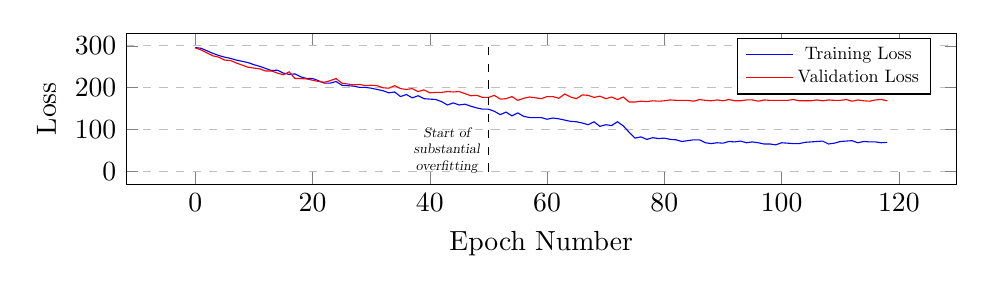
\begin{tikzpicture}
    \begin{axis}[
                height=3.5cm,
                width=\linewidth,
                xlabel={Epoch Number},
                ylabel={Loss},
                legend pos=north east,
                ymajorgrids=true,
                grid style=dashed,
                legend style={nodes={scale=0.65, transform shape}},
            ]
        %
        % TRAINING LOSS
        %
        \addplot[color=blue] coordinates {
            (0, 296) (1, 294) (2, 288) (3, 282) (4, 277) (5, 273) (6, 270) (7,
            266) (8, 263) (9, 260) (10, 255) (11, 251) (12, 246) (13, 241) (14,
            242) (15, 235) (16, 232) (17, 233) (18, 226) (19, 222) (20, 222)
            (21, 217) (22, 211) (23, 211) (24, 215) (25, 206) (26, 205) (27,
            204) (28, 201) (29, 201) (30, 199) (31, 196) (32, 193) (33, 188)
            (34, 190) (35, 179) (36, 184) (37, 176) (38, 181) (39, 174) (40,
            173) (41, 172) (42, 167) (43, 159) (44, 164) (45, 159) (46, 161)
            (47, 156) (48, 152) (49, 149) (50, 149) (51, 144) (52, 136) (53,
            142) (54, 133) (55, 140) (56, 132) (57, 129) (58, 129) (59, 129)
            (60, 125) (61, 128) (62, 126) (63, 123) (64, 120) (65, 119) (66,
            116) (67, 112) (68, 119) (69, 108) (70, 112) (71, 110) (72, 119)
            (73, 109) (74, 94) (75, 80) (76, 83) (77, 77) (78, 81) (79, 79) (80,
            80) (81, 77) (82, 76) (83, 72) (84, 74) (85, 76) (86, 76) (87, 69)
            (88, 67) (89, 69) (90, 68) (91, 72) (92, 71) (93, 73) (94, 69) (95,
            71) (96, 69) (97, 66) (98, 66) (99, 64) (100, 69) (101, 68) (102,
            67) (103, 67) (104, 70) (105, 71) (106, 72) (107, 73) (108, 66)
            (109, 68) (110, 72) (111, 73) (112, 74) (113, 69) (114, 72) (115,
            71) (116, 71) (117, 69) (118, 70)
        };
        \addlegendentry{Training Loss}
        %
        % VALIDATION LOSS
        %
        \addplot[color=red] coordinates {
            (0, 295) (1, 290) (2, 283) (3, 276) (4, 273) (5, 266) (6, 265) (7,
            259) (8, 254) (9, 249) (10, 247) (11, 245) (12, 240) (13, 240) (14,
            235) (15, 231) (16, 238) (17, 222) (18, 222) (19, 221) (20, 218)
            (21, 215) (22, 213) (23, 217) (24, 222) (25, 211) (26, 209) (27,
            207) (28, 208) (29, 205) (30, 206) (31, 205) (32, 200) (33, 199)
            (34, 205) (35, 198) (36, 196) (37, 198) (38, 191) (39, 195) (40,
            188) (41, 189) (42, 189) (43, 191) (44, 190) (45, 191) (46, 186)
            (47, 181) (48, 182) (49, 177) (50, 177) (51, 182) (52, 173) (53,
            174) (54, 179) (55, 170) (56, 175) (57, 178) (58, 176) (59, 174)
            (60, 179) (61, 179) (62, 175) (63, 185) (64, 178) (65, 174) (66,
            183) (67, 182) (68, 177) (69, 180) (70, 174) (71, 178) (72, 172)
            (73, 178) (74, 166) (75, 166) (76, 168) (77, 167) (78, 169) (79,
            168) (80, 169) (81, 171) (82, 170) (83, 170) (84, 170) (85, 168)
            (86, 172) (87, 170) (88, 169) (89, 171) (90, 169) (91, 172) (92,
            169) (93, 169) (94, 171) (95, 171) (96, 168) (97, 171) (98, 170)
            (99, 170) (100, 170) (101, 170) (102, 172) (103, 169) (104, 169)
            (105, 169) (106, 171) (107, 169) (108, 171) (109, 170) (110, 170)
            (111, 172) (112, 168) (113, 171) (114, 169) (115, 168) (116, 171)
            (117, 172) (118, 169) 
        };
        %
        % OVERFITTING LINE
        %
        \addplot[mark=none, dashed] coordinates {(50, 0) (50, 300)}
            node[midway, scale=0.5, yshift=-3em, xshift=-3em] {
                \parbox{5em}{\slshape\centering%
                    Start of substantial overfitting}
            };
        \addlegendentry{Validation Loss}
    \end{axis}
\end{tikzpicture}

%
    \caption{The losses on training data and validation data over training
        epochs}%
    \label{fig:loss-plot}
\end{figure}

\section{Conclusion and Further Work}
Considering the lack of pre-trained weights, coupled with the fast convergence
over a small training split, this CDNN is deemed to have achieved reasonable,
although certainly not maximal, test-accuracy. The modelled CDNN approximates
initial experiments by the VGG team \cite{Nilsback:2008}, albeit using a
differing DNN architecture. Within the space of convolutional DNNs, the
architecture described by Figure \ref{fig:network-architecture} is supported by
sensible design principles, although additional work should be undertaken to
determine the potential utility of adding hidden layers, or employing more
sophisticated LR schedulers \cite{Loshchilov:2017}.

\bibliographystyle{IEEEtran}
\bibliography{bibliography}
\vfill
\begin{center}
    \color{gray}%
    \begin{tabular}{c}
        \emph{Manuscript prepared with} \\[8pt]
        \huge\LaTeX \\[8pt]
        \huge Ti\textit{k}Z\\[8pt]
        \huge\texttt{IEEEtran}
    \end{tabular}
\end{center}
\end{document}

